\section{Bootstrap}
The {\bf bootstrap} is a statistical method for estimating standard errors and confidence sets of statistics, such as estimators.

\subsection{Non-parametric Bootstrap for Confidence Sets}\label{S:NPBootstrap}
Let $T_n := T_n((X_1,X_2,\ldots,X_n))$ be a statistic, i.e.~any function of the data $X_1,X_2,\ldots,X_n \overset{\IID}{\sim} F^*$.  Suppose we want to know its variance $\V_{F^*}(T_n)$, which clearly depends on the fixed and possibly unknown DF $F^*$.  

If our statistic $T_n$ is one with an analytically unknown variance, then we can use the bootstrap to estimate it.  The bootstrap idea has the following two basic steps:
\begin{enumerate}
\item[$\mathsf{Step~1}$:] Estimate $\V_{F^*}(T_n)$ with $\V_{\widehat{F}_n}(T_n)$.
\item[$\mathsf{Step~2}$:] Approximate $\V_{\widehat{F}_n}(T_n)$ using simulated data from the ``Bootstrap World.'' 
\end{enumerate}
For example, if $T_n=\overline{X}_n$, in $\mathsf{Step~1}$, $\V_{\widehat{F}_n}(T_n) = s_n^2/n$, where $s_n^2=n^{-1} \sum_{i=1}^n (x_i-\overline{x}_n)$ is the sample variance and $\overline{x}_n$ is the sample mean.  In this case,  $\mathsf{Step~1}$ is enough.  However, when the statistic $T_n$ is more complicated (e.g.~$T_n=\widetilde{X}_n = F^{[-1]}(0.5)$), the sample median, then we may not be able to find a simple expression for $\V_{\widehat{F}_n}(T_n)$ and may need $\mathsf{Step~2}$ of the bootstrap.

\begin{eqnarray}
\text{Real World Data come from} &  F^* \quad \implies X_1,X_2,\ldots,X_n & \implies 
T_n((X_1,X_2,\ldots,X_n))=t_n \notag \\
\text{Bootstrap World Data come from} & \widehat{F}_n \quad  \implies X^{\bullet}_1,X^{\bullet}_2,\ldots,X^{\bullet}_n & \implies 
T_n((X^{\bullet}_1,X^{\bullet}_2,\ldots,X^{\bullet}_n))=t^{\bullet}_n \notag
\end{eqnarray}

Observe that drawing an observation from the ECDF $\widehat{F}_n$ is equivalent to drawing one point at random from the original data (think of the indices $[n] := \{ 1,2,\ldots,n \}$ of the original data $X_1,X_2,\ldots,X_n$ being drawn according to the equi-probable $\demoivre(1/n,1/n,\ldots,1/n)$ RV on $[n]$).  Thus, to simulate $X^{\bullet}_1,X^{\bullet}_2,\ldots,X^{\bullet}_n$ from $\widehat{F}_n$, it is enough to drawn $n$ observations with replacement from $X_1,X_2,\ldots,X_n$.

In summary, the algorithm for Bootstrap Variance Estimation is:

\begin{enumerate}
\item[$\mathsf{Step~1}$:] Draw $X^{\bullet}_1,X^{\bullet}_2,\ldots,X^{\bullet}_n \sim \widehat{F}_n$
\item[$\mathsf{Step~2}$:] Compute $t_n^{\bullet} = T_n((X^{\bullet}_1,X^{\bullet}_2,\ldots,X^{\bullet}_n))$
\item[$\mathsf{Step~3}$:] Repeat $\mathsf{Step~1}$ and $\mathsf{Step~2}$ $B$ times, for some large $B$, say $B>1000$, to get $t_{n,1}^{\bullet}, t_{n,2}^{\bullet},\ldots,t_{n,B}^{\bullet}$
\item[$\mathsf{Step~4}$:] Several ways of estimating the bootstrap confidence intervals are possible:
\begin{enumerate}
\item The  $1-\alpha$ Normal-based bootstrap confidence interval is:
\[
C_n = [T_n - z_{\alpha/2} \widehat{se}_{boot}, T_n + z_{\alpha/2} \widehat{se}_{boot}] \ ,
\]
where the bootstrap-based standard error estimate is:
\[
\widehat{se}_{boot} = \sqrt{v_{boot}} = \sqrt{ \frac{1}{B} \sum_{b=1}^B \left(  t_{n,b}^{\bullet} - \frac{1}{B} \sum_{r=1}^B t_{n,r}^{\bullet} \right)^2}
\]
\item The $1-\alpha$ percentile-based bootstrap confidence interval is:\\
\[
C_n=[\widehat{G^{\bullet}}_{n}^{-1}(\alpha/2),\widehat{G^{\bullet}}_{n}^{-1}(1-\alpha/2)] ,
\]
where $\widehat{G^{\bullet}}_{n}$ is the empirical DF of the bootstrapped $t_{n,1}^{\bullet}, t_{n,2}^{\bullet},\ldots,t_{n,B}^{\bullet}$ and $\widehat{G^{\bullet}}_{n}^{-1}(q)$ is the $q^{\text{th}}$ sample quantile \eqref{E:qthSampleQuantile} of $t_{n,1}^{\bullet}, t_{n,2}^{\bullet},\ldots,t_{n,B}^{\bullet}$.
\end{enumerate}
\end{enumerate}

\begin{labwork} [Confidence Interval for Median Estimate of Inter Earth Quake Times]\label{LW:NZSIEQTimesMedianBootstrap}
Let us find the $95\%$ Normal-based bootstrap confidence interval as well as the  $95\%$ percentile-based bootstrap confidence interval for our plug-in estimate of the median of inter earth quake times from \hyperref[LW:PlugInEstimatesEarthQuakes]{Labwork~\ref*{LW:PlugInEstimatesEarthQuakes}} using the following script:
\VrbMf[label=NZSIEQTimesMedianBootstrap.m]{scripts/NZSIEQTimesMedianBootstrap.m}

We get the following output when we call the script file.
\begin{VrbM}
>> NZSIEQTimesMedianBootstrap
n =        6127
Medianhat =   25.5092
B =        1000
ans =        6127        1000
ConfInt95BootNormal =   24.4383   26.5800
ConfInt95BootPercentile =   24.4057   26.4742
\end{VrbM}
\end{labwork}

\begin{labwork}[Confidence Interval for Median Estimate of Web Login Data]
Find the $95\%$ Normal-based bootstrap confidence interval as well as the  $95\%$ percentile-based bootstrap confidence interval for our plug-in estimate of the median for each of the data arrays:
\[
\text{{\tt WebLogSeconds20071001035730} and {\tt WebLogSeconds20071002035730} .}
\]
Once again, the arrays can be loaded into memory by following the commands in the first $13$ lines of the script file {\tt WebLogDataProc.m} of \hyperref[DA:WebLogs]{Section~\ref*{DA:WebLogs}}.  Produce four intervals (two for each data-set).  Do the confidence intervals for the medians for the two days intersect?
\begin{VrbM}
>> WebLogDataProc % load in the data
>> Medianhat = median(WebLogSeconds20071001035730) % plug-in estimate of median
Medianhat =       37416
>> % store the length of data array
>> K=length(WebLogSeconds20071001035730) 
K =       56485
>> B= 1000 % Number of Bootstrap replications
B =        1000
>> BootstrappedDataSet = WebLogSeconds20071001035730([ceil(K*rand(K,B))]); 
>> size(BootstrappedDataSet) % dimension of the BootstrappedDataSet
ans =       56485        1000
>> BootstrappedMedians=median(BootstrappedDataSet); % get the statistic in Bootstrap world
>> % 95% Normal based Confidence Interval
>> SehatBoot = std(BootstrappedMedians); % std of BootstrappedMedians
>> % 95% C.I. for median from Normal approximation
>> ConfInt95BootNormal = [Medianhat-1.96*SehatBoot, Medianhat+1.96*SehatBoot] 
ConfInt95BootNormal =    37242    37590
>> % 95% Percentile based Confidence Interval
ConfInt95BootPercentile = ...
    [qthSampleQuantile(0.025,sort(BootstrappedMedians)),...
    qthSampleQuantile(0.975,sort(BootstrappedMedians))]
ConfInt95BootPercentile =   37239    37554
\end{VrbM}
\end{labwork}

\begin{labwork}[Confidence interval for correlation]\label{LW:LSATGPACorrBoot}
Here is a classical data set used by Bradley Efron (the inventor of bootstrap) to illustrate the method.  The data are LSAT (Law School Admission Test in the U.S.A.) scores and GPA of fifteen individuals.

Thus, we have bivariate data of the form $(Y_i,Z_i)$, where $Y_i={\rm LSAT}_i$ and $Z_i={\rm GPA}_i$.  For example, the first individual had an LSAT score of  $y_1=576$ and a GPA of $z_1=3.39$ while the fifteenth individual had an LSAT score of $y_{15}=594$ and a GPA of $z_{15}=3.96$.  We supose that the bivariate data $(Y_i,Z_i) \overset{IID}{\sim} F^*$, such that $F^* \in \{ \text{all bivariate DFs} \}$.  This is a bivariate non-parametric experiment.  The bivariate data are plotted in Figure .


The law school is interested in the correlation between the GPA and LSAT scores:
$$
\theta^* = \frac{\int \int (y-\E(Y))(z-\E(Z))dF(y,z)}{\sqrt{\int (y-\E(Y))^2 dF(y) \int (z-\E(Z))^2 dF(z)}}
$$
The plug-in estimate of the population correlation $\theta^*$ is the sample correlation:
$$
\widehat{\Theta}_n = \frac{\sum_{i=1}^n(Y_i-\overline{Y}_n)(Z_i-\overline{Z}_n)}{\sqrt{\sum_{i=1}^n(Y_i-\overline{Y}_n)^2 \sum_{i=1}^n(Z_i-\overline{Z}_n)^2}}
$$ 
\VrbMf[label=LSATGPACorrBootstap.m]{scripts/LSATGPACorrBootstap.m}

We get the following output when we call the script file.
\begin{VrbM}
>> LSATGPACorrBootstap
SampleCorrelation =    0.5459
ConfInt95BootNormal =    0.1770    0.9148
ConfInt95BootPercentile =    0.2346    0.9296
\end{VrbM}

\begin{figure}
\caption{Data from Bradley EfronÕs LSAT and GPA scores for fifteen individuals (left).  The confidence interval of the sample correlation, the plug-in estimate of the population correlation, is obtained from the sample correlation of one thousand bootstrapped data sets (right).\label{F:LSATGPACorrBootstrap}}
\begin{center}
\makebox{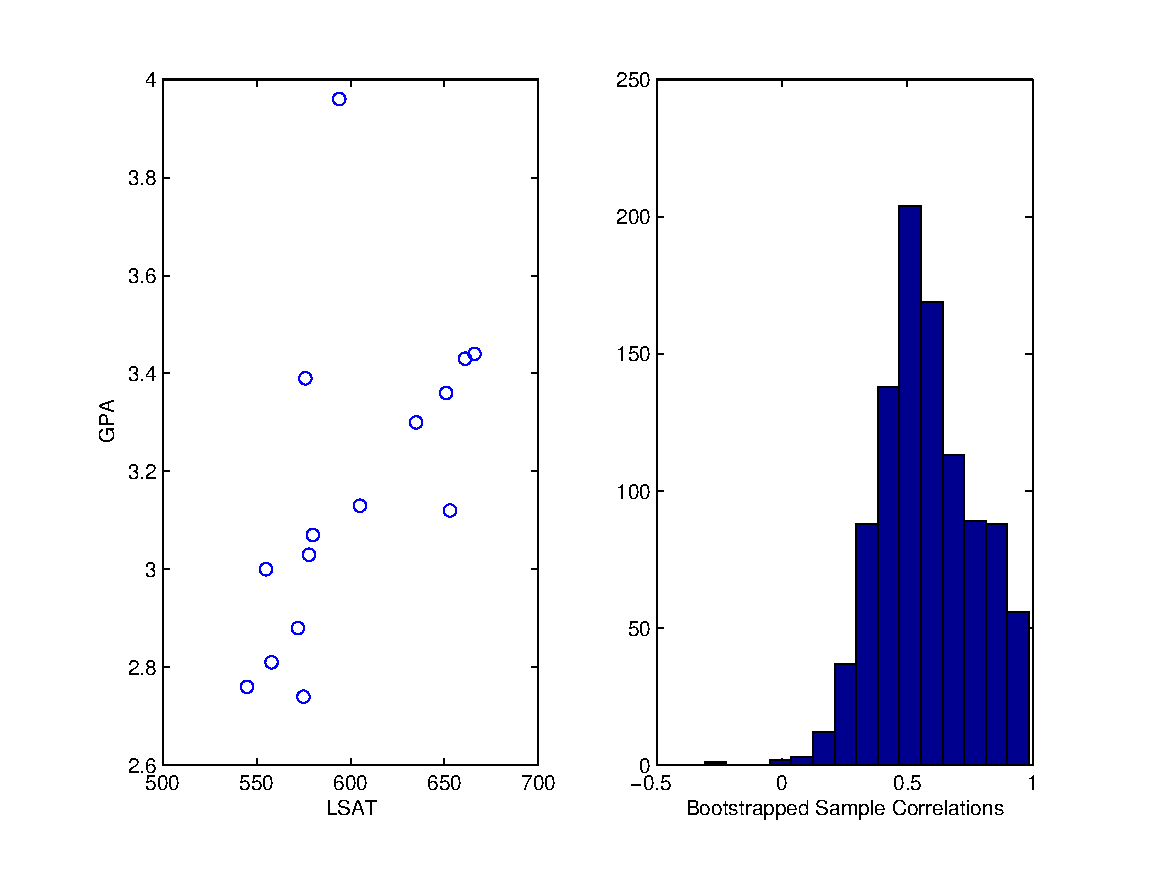
\includegraphics[width=4.5in]{figures/LSATGPACorrBootstrap}}
\end{center}
\end{figure}

\end{labwork}

\subsection{Parametric Bootstrap for Confidence Sets}\label{S:PBootstrap}

The {\bf bootstrap} may also be employed for estimating standard errors and confidence sets of statistics, such as estimators, even in a parametric setting.  This is much easier than the the variance calculation based on Fisher Information and/or the Delta method.  

The only difference in the {\bf parametric bootstrap} as opposed to the {\bf non-parametric bootstrap} we saw earlier is that our statistic of interest $T_n := T_n((X_1,X_2,\ldots,X_n))$ is a function of the data: 
$$X_1,X_2,\ldots,X_n \overset{\IID}{\sim} F(x;\theta^*) \enspace .$$
That is, our data come from a parametric distribution $F(x;\theta^*)$ and we want to know the variance of our statistic $T_n$, i.e.~$\V_{\theta^*}(T_n)$.  

The parametric bootstrap concept has the following two basic steps:
\begin{enumerate}
\item[$\mathsf{Step~1}$:] Estimate $\V_{\theta^*}(T_n)$ with $\V_{\widehat{\theta}_n}(T_n)$, where $\widehat{\theta}_n$ is an estimate of $\theta^*$ based on maximum likelihood or the method of moments.
\item[$\mathsf{Step~2}$:] Approximate $\V_{\widehat{\theta}_n}(T_n)$ using simulated data from the ``Bootstrap World.'' 
\end{enumerate}
For example, if $T_n=\overline{X}_n$, the sample mean, then in $\mathsf{Step~1}$, $\V_{\widehat{\theta}_n}(T_n) = n^{-1} \sum_{i=1}^n (x_i-\overline{x}_n)$ is the sample variance.  Thus, in this case,  $\mathsf{Step~1}$ is enough.  However, when the statistic $T_n$ is more complicated, say $T_n=\widetilde{X}_n = F^{[-1]}(0.5)$, the sample median, then we may not be able to write down a  simple expression for $\V_{\widehat{\theta}_n}(T_n)$ and may need $\mathsf{Step~2}$ of the bootstrap.
\begin{eqnarray}
{\scriptsize \text{Real World Data come from}} &  F(\theta^*) \quad \implies X_1,X_2,\ldots,X_n & \implies 
T_n((X_1,X_2,\ldots,X_n))=t_n \notag \\
{\scriptsize \text{Bootstrap World Data come from}} & F(\widehat{\theta}_n) \quad  \implies X^{\bullet}_1,X^{\bullet}_2,\ldots,X^{\bullet}_n & \implies 
T_n((X^{\bullet}_1,X^{\bullet}_2,\ldots,X^{\bullet}_n))=t^{\bullet}_n \notag
\end{eqnarray}
To simulate $X^{\bullet}_1,X^{\bullet}_2,\ldots,X^{\bullet}_n$ from $F(\widehat{\theta}_n)$, we must have a simulation algorithm that allows us to draw IID samples from $F(\theta)$, for instance the inversion sampler.  In summary, the algorithm for Bootstrap Variance Estimation is:
\begin{enumerate}
\item[$\mathsf{Step~1}$:] Draw $X^{\bullet}_1,X^{\bullet}_2,\ldots,X^{\bullet}_n \sim F(\widehat{\theta}_n)$
\item[$\mathsf{Step~2}$:] Compute $t_n^{\bullet} = T_n((X^{\bullet}_1,X^{\bullet}_2,\ldots,X^{\bullet}_n))$
\item[$\mathsf{Step~3}$:] Repeat $\mathsf{Step~1}$ and $\mathsf{Step~2}$ $B$ times, for some large $B$, say $B\geq1000$, to get $t_{n,1}^{\bullet}, t_{n,2}^{\bullet},\ldots,t_{n,B}^{\bullet}$
\item[$\mathsf{Step~4}$:] We can estimate the bootstrap confidence intervals in several ways:
\begin{enumerate}
\item The  $1-\alpha$ normal-based bootstrap confidence interval is:
\[
C_n = [T_n - z_{\alpha/2} \widehat{se}_{boot}, T_n + z_{\alpha/2} \widehat{se}_{boot}] \ ,
\]
where the bootstrap-based standard error estimate is:
\[
\widehat{se}_{boot} = \sqrt{v_{boot}} = \sqrt{ \frac{1}{B} \sum_{b=1}^B \left(  t_{n,b}^{\bullet} - \frac{1}{B} \sum_{r=1}^B t_{n,r}^{\bullet} \right)^2}
\]
\item The $1-\alpha$ percentile-based bootstrap confidence interval:\\
\[
C_n=[\widehat{G^{\bullet}}_{n}^{-1}(\alpha/2),\widehat{G^{\bullet}}_{n}^{-1}(1-\alpha/2)] ,
\]
where $\widehat{G^{\bullet}}_{n}$ is the empirical DF of the bootstrapped $t_{n,1}^{\bullet}, t_{n,2}^{\bullet},\ldots,t_{n,B}^{\bullet}$ and $\widehat{G^{\bullet}}_{n}^{-1}(q)$ is the $q^{\text{th}}$ sample quantile \eqref{E:qthSampleQuantile} of $t_{n,1}^{\bullet}, t_{n,2}^{\bullet},\ldots,t_{n,B}^{\bullet}$.
\end{enumerate}
\end{enumerate}

Let us apply the bootstrap method to the previous problem of estimating the standard error of the coefficient of variation from $n=100$ samples from $\normal(100,10^2)$ RV.  The confidence intervals from bootstrap-based methods are similar to those from the Delta method.
{\VrbMf[label=CoeffOfVarNormalBoot.m]{scripts/CoeffOfVarNormalBoot.m}}
\begin{VrbM}
>> CoeffOfVarNormal
Muhat =  100.3117
Sigmahat =   10.9800
Psihat =    0.1095
Sehat =    0.0077
ConfInt95DeltaMethod =    0.0943    0.1246
ConfInt95BootNormal =    0.0943    0.1246
ConfInt95BootPercentile =    0.0946    0.1249
\end{VrbM}
